\documentclass[a4paper]{article}
\usepackage{amsmath,amssymb,float,geometry,graphicx,xcolor}
\geometry{left=3.5cm,right=3.5cm,top=3.3cm,bottom=3.3cm}
\renewcommand\thesection{\arabic{section}}
\begin{document}
\begin{center}
\huge
\textbf{VE320\\Intro to Semiconductor Devices\\}
\Large
\vspace{30pt}
\uppercase{Homework 7}\\
\vspace{5pt}\today\\
\vspace{5pt}
Yihua Liu 518021910998
\vspace{5pt}
\rule[-10pt]{.97\linewidth}{0.05em}
\end{center}
1. (a) Substituting $N_c=2.8\times10^{19}\ \mathrm{cm^{-3}}$ for $N_c$, $5\times10^{15}\ \mathrm{cm^{-3}}$ for $N_d$,
$$\phi_n=\frac{kT}{e}\ln{\bigg(\frac{N_c}{N_d}\bigg)}=0.2231\ \mathrm{V}.$$
The built-in potential barrier $V_{bi}$ is
$$V_{bi}=\phi_{B0}-\phi_n=0.4269\ \mathrm{V}.$$

(b) When $N_d=10^{16}\ \mathrm{cm^{-3}}$, since the value of the Schottky barrier height $\phi_{B0}$ has no relation to the doping concentration $N_d$, it will remain the same as
$$\phi_{B0}=0.65\ \mathrm{V}.$$
$$\phi_n=\frac{kT}{e}\ln{\bigg(\frac{N_c}{N_d}\bigg)}=0.2052\ \mathrm{V}.$$
The built-in potential barrier $V_{bi}$ is
$$V_{bi}=\phi_{B0}-\phi_n=0.4448\ \mathrm{V}.$$
The value of $\phi_{B0}$ remains the same, while the value of $V_{bi}$ increases.

(c) When $N_d=10^{15}\ \mathrm{cm^{-3}}$, for the same reason,
$$\phi_{B0}=0.65\ \mathrm{V}.$$
$$\phi_n=\frac{kT}{e}\ln{\bigg(\frac{N_c}{N_d}\bigg)}=0.2647\ \mathrm{V}.$$
The built-in potential barrier $V_{bi}$ is
$$V_{bi}=\phi_{B0}-\phi_n=0.3853\ \mathrm{V}.$$
The value of $\phi_{B0}$ remains the same, while the value of $V_{bi}$ decreases.

2. (a) From Figure 9.5 we read that $\phi_m=4.65$ V and the Schottky barrier is
$$\phi_{B0}=0.63\ \mathrm{V}.$$
The reverse-saturation current density $J_{sT}$ is
$$J_{sT}=A^*T^2\exp{\bigg(\frac{-e\phi_{B0}}{kT}\bigg)}=120\times300^2\times\mathrm{e}^{\frac{-0.63e}{300k}}=2.818\times10^{-4}\ \mathrm{A/cm^2}.$$
The reverse-saturation current $I_{sT}$ is
$$I_{sT}=AJ_{sT}=2.818\times10^{-8}\ \mathrm{A}.$$
When $I=10\ \mu\mathrm{A}=10^{-5}\ \mathrm{A}$, the forward-bias voltage is
$$V_a=\frac{kT}{e}\ln{\bigg(\frac{I}{I_{sT}}+1\bigg)}=0.1519\ \mathrm{V}.$$
When $I=100\ \mu\mathrm{A}=10^{-4}\ \mathrm{A}$, the forward-bias voltage is
$$V_a=\frac{kT}{e}\ln{\bigg(\frac{I}{I_{sT}}+1\bigg)}=0.2113\ \mathrm{V}.$$
When $I=1\ \mathrm{mA}=10^{-3}\ \mathrm{A}$, the forward-bias voltage is
$$V_a=\frac{kT}{e}\ln{\bigg(\frac{I}{I_{sT}}+1\bigg)}=0.2709\ \mathrm{V}.$$

(b) Assuming $T=350$ K, the reverse-saturation current $I_{sT}$ is
$$I_{sT}=AJ_{sT}=AA^*T^2\exp{\bigg(\frac{-e\phi_{B0}}{kT}\bigg)}=1.247\times10^{-6}\ \mathrm{A}.$$
When $I=10\ \mu\mathrm{A}=10^{-5}\ \mathrm{A}$, the forward-bias voltage is
$$V_a=\frac{kT}{e}\ln{\bigg(\frac{I}{I_{sT}}+1\bigg)}=0.06634\ \mathrm{V}.$$
When $I=100\ \mu\mathrm{A}=10^{-4}\ \mathrm{A}$, the forward-bias voltage is
$$V_a=\frac{kT}{e}\ln{\bigg(\frac{I}{I_{sT}}+1\bigg)}=0.1326\ \mathrm{V}.$$
When $I=1\ \mathrm{mA}=10^{-3}\ \mathrm{A}$, the forward-bias voltage is
$$V_a=\frac{kT}{e}\ln{\bigg(\frac{I}{I_{sT}}+1\bigg)}=0.2017\ \mathrm{V}.$$

3. (a) From the I-V characteristic, we have
$$I=I_{sT}\bigg[\exp{\bigg(\frac{eV_a}{kT}\bigg)-1}\bigg],$$
thus, the forward-bias voltage of Schottky diode is
$$V_{a1}=\frac{kT}{e}\ln{\bigg(\frac{I}{I_{sT1}}+1\bigg)}.$$
Substituting $150\ \mu\mathrm{A}=1.5\times10^{-4}\ \mathrm{A}$ for $I$, $AJ_{sT1}=8\times10^{-4}\times6\times10^{-9}=4.8\times10^{-12}$ A, the forward-bias voltage of Schottky diode is
$$V_{a1}=0.4461\ \mathrm{V}.$$
The forward-bias voltage of pn junction diode is
$$V_{a2}=\frac{kT}{e}\ln{\bigg(\frac{I}{I_{sT2}}+1\bigg)}.$$
Substituting $150\ \mu\mathrm{A}=1.5\times10^{-4}\ \mathrm{A}$ for $I$, $AJ_{sT1}=8\times10^{-4}\times8\times10^{-13}=6.4\times10^{-16}$ A, the forward-bias voltage of pn junction diode is
$$V_{a2}=0.6768\ \mathrm{V}.$$

(b) Similar to (a), when $I=700\ \mu\mathrm{A}=7\times10^{-4}\ \mathrm{A}$, the forward-bias voltage of Schottky diode is
$$V_{a1}=\frac{kT}{e}\ln{\bigg(\frac{I}{I_{sT1}}+1\bigg)}=0.4860\ \mathrm{V}.$$
The forward-bias voltage of pn junction diode is
$$V_{a2}=\frac{kT}{e}\ln{\bigg(\frac{I}{I_{sT2}}+1\bigg)}=0.7166\ \mathrm{V}.$$

(c) When $I=1.2\ \mathrm{mA}=1.2\times10^{-3}\ \mathrm{A}$, the forward-bias voltage of Schottky diode is
$$V_{a1}=\frac{kT}{e}\ln{\bigg(\frac{I}{I_{sT1}}+1\bigg)}=0.4999\ \mathrm{V}.$$
The forward-bias voltage of pn junction diode is
$$V_{a2}=\frac{kT}{e}\ln{\bigg(\frac{I}{I_{sT2}}+1\bigg)}=0.7306\ \mathrm{V}.$$

4. (a) (i) The resistance at junction is
$$R=\frac{R_c}{A}=\frac{5\times10^{-5}}{10^{-5}}=5\ \Omega.$$
When the current $I=1\ \mathrm{mA}=1\times10^{-3}\ \mathrm{A}$, the voltage across the junction is
$$V=IR=1\times10^{-3}\times5=5\times10^{-3}\ \mathrm{V}.$$

(ii) When $I=100\ \mu\mathrm{A}=1\times10^{-4}\ \mathrm{A}$, the voltage across the junction is
$$V=IR=1\times10^{-4}\times5=5\times10^{-4}\ \mathrm{V}.$$

(b) (i) Similar to (a), the resistance at junction is
$$R=\frac{R_c}{A}=\frac{5\times10^{-5}}{10^{-6}}=50\ \Omega.$$
When the current $I=1\ \mathrm{mA}=1\times10^{-3}\ \mathrm{A}$, the voltage across the junction is
$$V=IR=1\times10^{-3}\times50=5\times10^{-2}\ \mathrm{V}.$$

(ii) When the current $I=100\ \mu\mathrm{A}=1\times10^{-4}\ \mathrm{A}$, the voltage across the junction is
$$V=IR=1\times10^{-4}\times50=5\times10^{-3}\ \mathrm{V}.$$

5. (a) We have $\phi_s=\chi_s+(E_c-E_F)_\text{FB}$,
$$E_c-E_F=-\frac{kT}{e}\ln{\bigg(\frac{n_0}{N_c}\bigg)}=0.5519\ \mathrm{V},$$
thus $\phi_s=\chi_s+(E_c-E_F)_\text{FB}>4.5518\ \mathrm{V}>\phi_m=4.2\ \mathrm{V}$.

The energy-band diagram for zero bias for the case when no space charge region exists at the junction is
\begin{figure}[H]
    \centering
    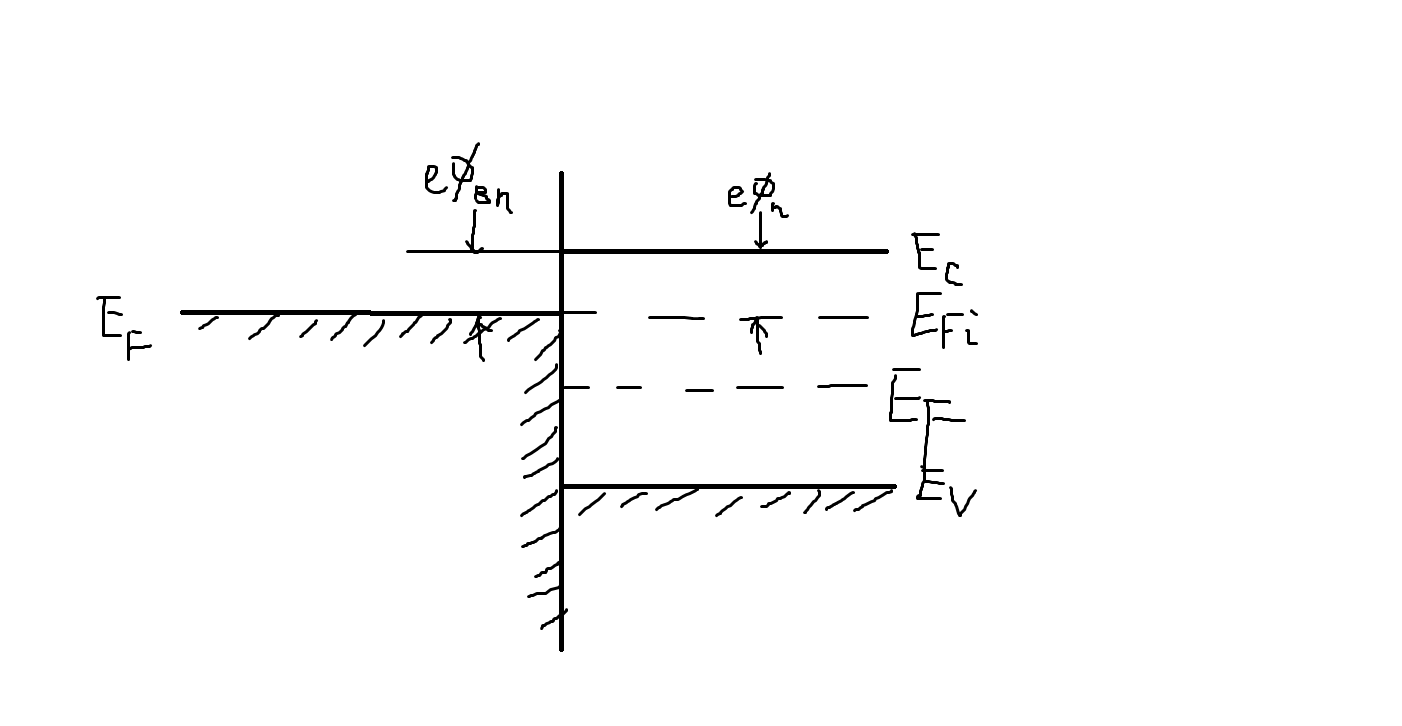
\includegraphics[width=1\textwidth]{1.png}
    \caption{5(a).}
\end{figure}
(b) The schottky barrier is
$$\phi_{Bn}=\phi_m-\chi_s=4.2-4.0=0.2\ \mathrm{V}.$$
% Since $V_{bi}=\phi_{B0}-\phi_n$,
$$\phi_n=\phi_{Bn}=0.2\ \mathrm{V}.$$
On the other hand,
$$\phi_n=\frac{kT}{e}\ln{\bigg(\frac{N_c}{N_d}\bigg)}=\frac{300k}{e}\ln{\bigg(\frac{2.8\times10^{19}}{N_d}\bigg)}=0.2\ \mathrm{V}.$$
Solving the equation,
$$N_d=1.223\times10^{16}\ \mathrm{cm^{-3}}.$$

(c) From (b) we have the potential barrier height seen by electrons in the metal moving into the semiconductor is 0.2 V.

6. (a) The thermal equilibrium energy-band diagram is
\begin{figure}[H]
    \centering
    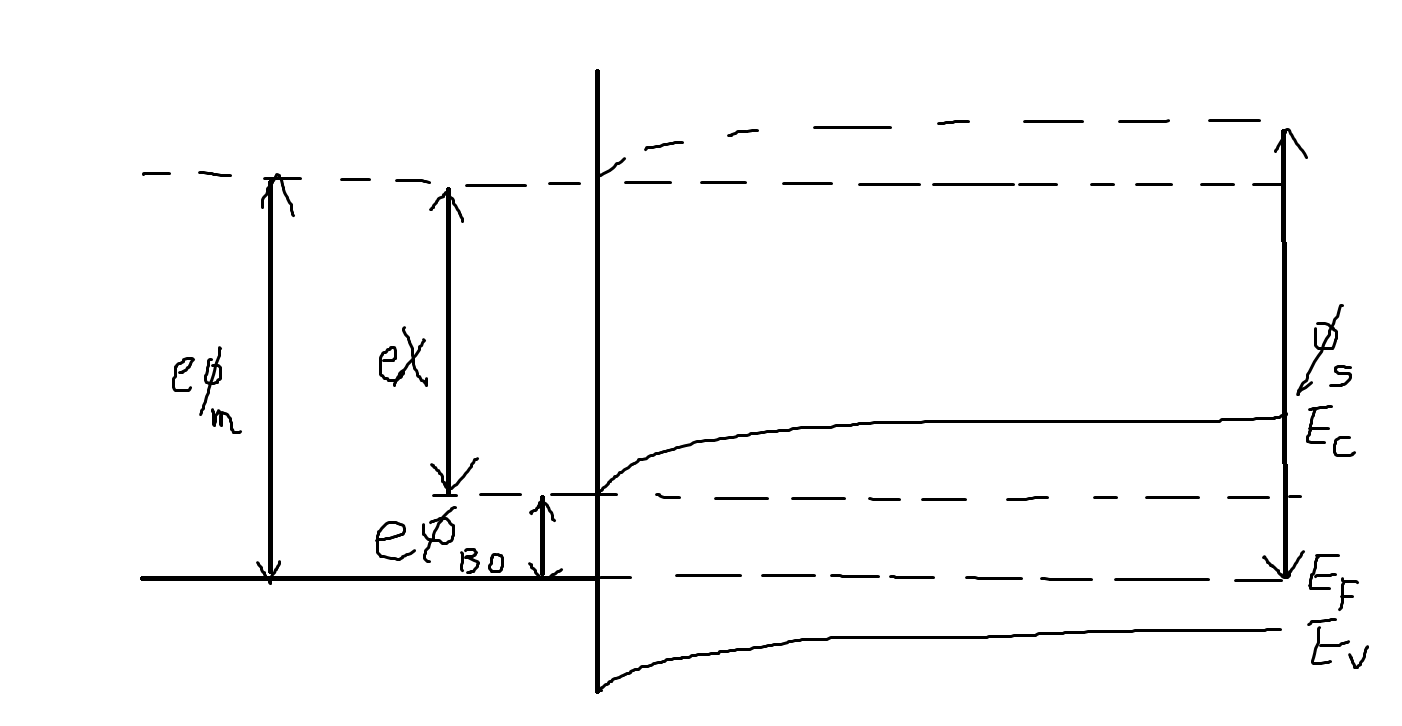
\includegraphics[width=1\textwidth]{2.png}
    \caption{6(a).}
\end{figure}

(b)
$$\phi_{B0}=\phi_m-\chi_s=4.3-4.0=0.3\ \mathrm{eV}.$$

(c)
\begin{figure}[H]
    \centering
    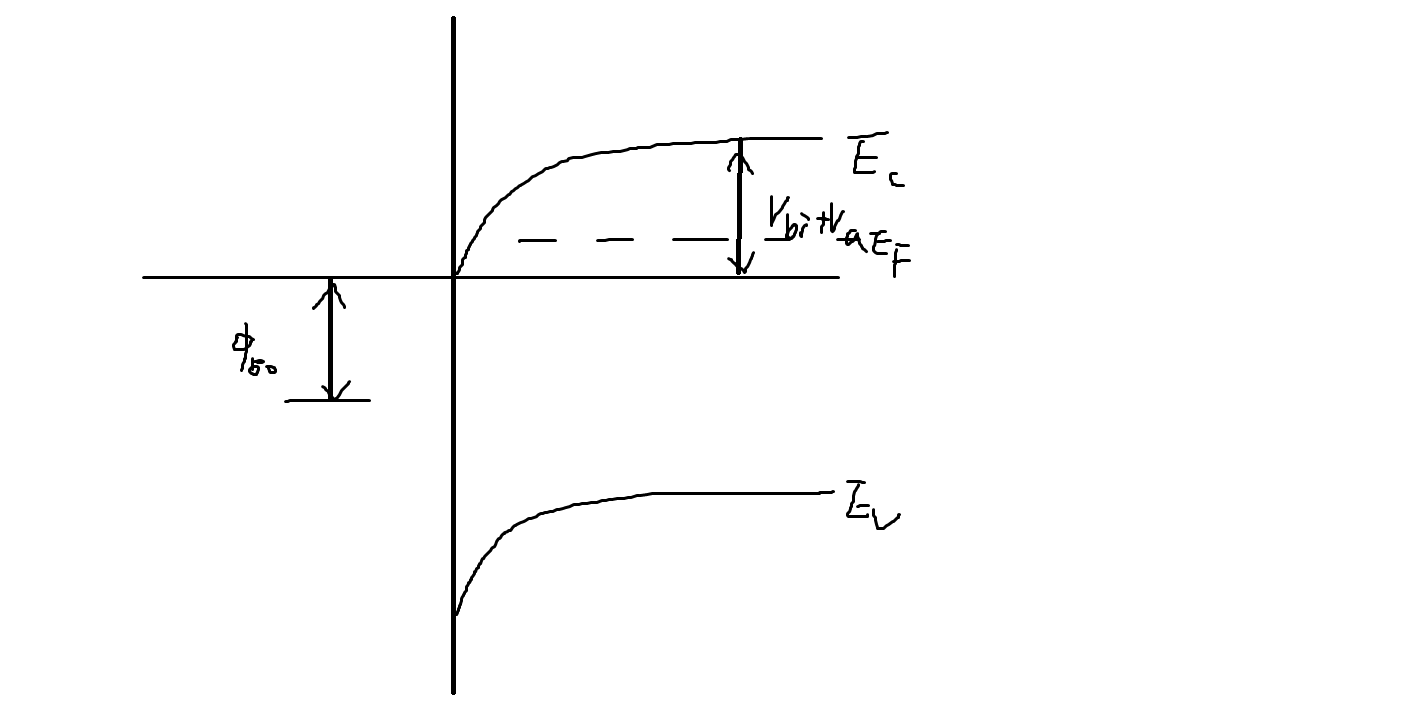
\includegraphics[width=1\textwidth]{3.png}
    \caption{6(c).}
\end{figure}

(d)
\begin{figure}[H]
    \centering
    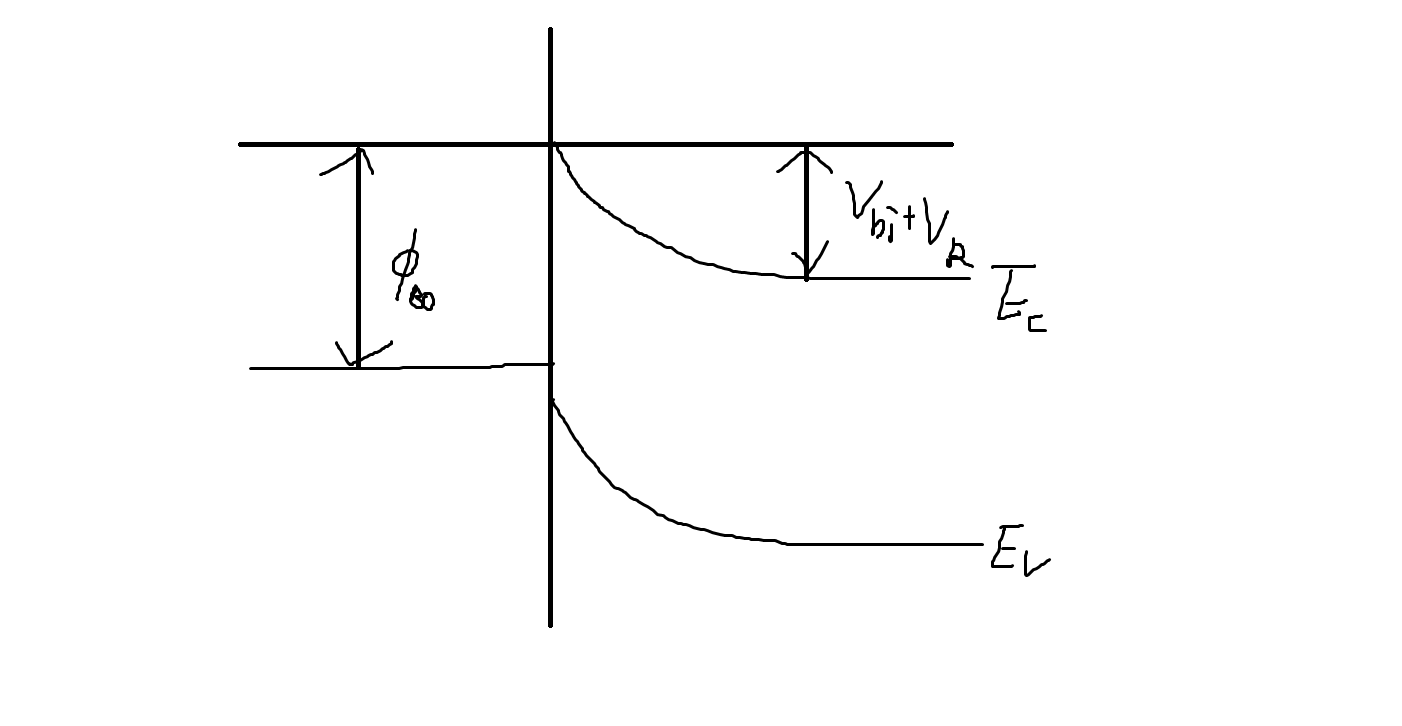
\includegraphics[width=1\textwidth]{4.png}
    \caption{6(d).}
\end{figure}
\end{document}